In this section the experimental validation is presented.
%
Specifically, we show that by explicitly controlling the diversity in DE, results of state-of-the-art algorithms
are improved further.
%
Particularly, the benchmarks of \CEC{} 2016 and \CEC{} 2017 are considered.
%
Each one of them is composed of thirty different problems.
%
The state-of-the-art is composed by the algorithms that attained the first places of each year competition.
%
Thus, the algorithms considered from the \CEC{} 2016 are UMOEAs-II \cite{elsayed2016testing} and L-SHADE-EpSin \cite{awad2016ensemble} that achieved 
the first and second place respectively.
%
Similarly, the top algorithms from \CEC{} 2017 are EBOwithCMAR \cite{kumar2017improving} and jSO \cite{brest2017single}.
%
It is interesting to remark that EBOwithCMAR is considered as an improvement of the UMOEAs-II.
%
Additionally, jSO and L-SHADE-EpSin belong to the SHADE's family.
%
All these algorithms are tested with both benchmarks as it is suggested by \cite{molina2017analysis}.

Given that all of them are stochastic algorithms, each execution was repeated 51 times with different seeds.
%
In every case, the stopping criterion was set to $25,000,000$ functions evaluations.
%
We performed our evaluation following the guidelines of \CEC{} benchmark competitions.
%
Thus, if the gap between the values of the best solution found and the optimal solution was $10^{-8}$ or smaller, the error is treated as $0$.
%
%The minimal tolerance to consider a determined problem solved is $1e-8$, hence if the difference of the optimal obtained and the true optinal is below this tolerance then the error is zero.
%
The parameterization indicated by the authors was used in every algorithm and it is as follows:
\begin{itemize}
\item \textbf{EBOwithCMAR}: For EBO, the maximum population size of $S_1 = 18D$, minimum population size of $S_1 = 4$, maximum population size of $S_2 = 146.8D$, minimum population size of $S_2 = 10$, historical memory size H=$6$. For CMAR Population size $S_3 = 4 + 3log(D)$, $\sigma=0.3$, CS = $50$, probability of local search $pl = 0.1$ and $cfe_{ls} = 0.4* FE_{max}$.
\item \textbf{UMOEAs-II}: For MODE, maximum population size of $S_1 = 18D$, minimum population size of $S_1 = 4$, size memory H=$6$. For CMA-ES Population size $S_2 = 4 + \lfloor 3log(D) \rfloor$, $\mu=\frac{PS}{2}$, $\sigma=0.3$, CS = $50$. For local search, $cfe_{ls} = 0.2 * FE_{max}$.
\item \textbf{jSO}: Maximum population size = $25log(D)\sqrt{D}$, historical memory size H= $5$, initial mutation memory $M_F = 0.5$, initial probability memory $M_{CR} = 0.8$, minimum population size = $4$, initial p-best = $0.25*N$, final p-best = $2$.
\item \textbf{L-SHADE-EpSin}: Maximum population size = $25log(D)\sqrt{D}$, historical memory size H= $5$, initial mutation memory $M_F = 0.5$, initial probability memory $M_{CR} = 0.5$, initial memory frequency $\mu_F = 0.5$, minimum population size = $4$, initial p-best = $0.25*N$, final p-best = $2$, generations of local search $G_{LS}=250$.
\item \textbf{ \textsc{DE-EDM} }: $D_I = 0.3$, population size = $250$.
\end{itemize}
%

Our experimental analyses have been performed in base of the difference between the optimal solution and the best obtained solution.
%
In order to statistically compare the results, a similar guideline than the one proposed in~\cite{Joel:StatisticalTest} was used. 
%
First a Shapiro-Wilk test was performed to check whatever or not the values of the results followed a Gaussian distribution. 
%
If, so, the Levene test was used to check for the homogeneity of the variances. 
%
If samples had equal variance, an ANOVA test was done; if not, a Welch test was performed. 
%
For non-Gaussian distributions, the non parametric Kruskal-Wallis test was used to test whether samples are drawn from the same distribution. 
%
An algorithm $X$ is said to win algorithm $Y$ when the differences between them are statistically significant, and the mean and median obtained by $X$ are higher 
than the mean and median achieved by $Y$.

In tables \ref{tab:Summary_CEC2016} and \ref{tab:Summary_CEC2017} a summary of the results obtained for \CEC{} 2016 and \CEC{} 2017 are shown, respectively.
%
The column tagged with ``Always Solved'' shows the number of functions where a zero error was obtained in the 51 runs.
%
Additionally, column tagged with ``At least one time solved'' shows the number of functions that were solved to optimality at least in one run.
%
Practically all functions (28 of them) of the \CEC{} 2017 benchmark were solved with our proposal at least one time.
%
Additionally, 21 functions of the \CEC{} 2016 were also solved.
%
This constrast with the results obtained by state-of-the-art algorithms.
%
They were able to reach optimal values in significantly less functions.
%
In order to confirm the superioriy of \DEEDM{}, pair-wise statisticall test were used.
%
The column tagged with the symbol $\uparrow$ shows the number of times that the superiority of each method could be confirmed, whereas
the column tagged with the symbol $\downarrow$ count the number of cases where the method was inferior.
%
Finally, the number comparisons where differences were not significant are shown in the column tagged with the symbol $\longleftrightarrow$.

%TODO: Poner frases del tipo que fue el que mas veces ganó y el que menos veces perdió
%The statistical tests indicate that the diversity DE algorithm provides significantly better results that the state-of-the-art algorithms in both benchmarks.
%
%Even though out proposal loses with the functions $\{f_6, f_7, f_{13}, f_{14}, f_{28}\}$ and $\{ f_{12}, f_{16}, f_{18} \}$ in \CEC{} 2016 and \CEC{} 2017 respectively,it provides acceptable quality solutions, that in some problems reach the optimal region.
%
%Based in a preliminary study these functions were solved at least one time with different configurations (tuning the $D_I$ and population size).

%TODO: pasar el score a la última columna y decir que además del análisis se realizó el análisis propuesto en la competición, que se base
%en calcular un score...
%TODO: remarcar que la nueva propuesta consigue score 100 en ambos casos, confirmando la superioridad que se vio con el resto de análisis realizados, decir
%que significa tener score 100

Based in the guideline of the \CEC{}, the ``Score'' is computed as follows.
%
The evaluation method combines two scores defined in the equation (\ref{eqn:total_scores}).
%
Thus the final score is composed by the sum $Score = Score_1 + Score_2$.
%
\begin{equation}\label{eqn:total_scores}
\begin{split}
Score_1 &= \left (1 - \frac{SE - SE_{min}}{SE} \right) \times 50, \\
Score_2 &= \left  (1 - \frac{SR - SR_{min}}{SR} \right ) \times 50, \\
\end{split}
\end{equation}
Here, $SE_{min}$ is the minimal sum of errors from all the algorithms, and $SE$ is the sum of error values $SE = \sum_{i=1}^{30} error\_f_i$.
%
Also, $SR_{min}$ is the minimal sum of ranks from all the algorithms, namely the sum of each rank in each function for the considered algorithms $SE = \sum_{i=1}^{30} error\_f_i$.
%
Based in the final score the results provided for our proposal are superior in both years.
%
On the other hand, the UMOEAs-II has the second best score in \CEC{} 2017, and the EBOwithCMAR has the second best score in the \CEC{} 2016.
%
The same effect occurs in the third place with the SHADE's algorithms jSO and L-SHADE-EpSin.
%
Thus, its evident that the performance of the algorithms is different with long-term executions.
%
Also, this might be a highlight that the SHADE's algorithms are improved by the multi-operator algorithms.
%
However, it seems that the multi-operator could be sensible with the parameterization.
%
So, the winners of the \CEC{} 2016 outperform to the winners of the \CEC{} 2017 in long-term, and the winners of the \CEC{} 2017 outperform to the winners of the \CEC{} 2016.
%

%TODO: quitar todo lo que tenga que ver con análisis de lo que hacen internamente los otros algoritmos. No estamos cambiando nada asi
%que en eso no nos metemos. Vamos al grano!
Based in several experiments one drawback of the L-SHADE-EpSin and EBOwithCMAR resides in the strategy to adapt the mutation factor $F$.
%
These algorithms take into account the elapsed evaluations to adapt the mutation factor, however this strategy does not considers long-term executions.
%
Thus, the adaptation of this parameter is unstable.
%
In several experiments we try tuning the mutation factor, however the results were not significantly different. 
%
Broadly speaking, the results of the state-of-the-art shows that each algorithm was specifically tuned to short-term executions and for their respectively benchmark.
%

%TODO: Poner Dado que nuestra novedad está en el control de la diversidad, para comprender mejor el comportamiento de la propuesta...

The mechanism of the \DEEDM{} should maintain the diversity properly, with the aim of have a better understanding of the methodology proposed, in the figure \ref{fig:diversity} is showed the diversity through the time elapsed of \DEEDM{} with two functions: $f_1$ and $f_{30}$ respectively.
%
While the first function is easily solved, the second is one of the most difficult.
%
In the left side are showed the Elite vectors, although there are not constraints in the Elite vector to lost the diversity, it seems that in both functions $f_1$ and $f_{30}$ the diversity is implicitly maintained.
%
On the other hand the trial vectors maintain the diversity a is desired ( i.e. until the $95\%$ of the total function evaluations).

\begin{figure}[t]
\centering
\begin{tabular}{cc}
   \includegraphics[scale=0.23, angle=-90]{img/Diversity_Elite.eps} 
   \includegraphics[scale=0.23, angle=-90]{img/Diversity_Trial.eps} 
\end{tabular}
\caption{ Average \DCN{} of the 51 executions with the problems $f_1$ and $f_{30}$ (\CEC{} 2016 and \CEC{} 2017). The initial distance factor considered corresponds to $D_I=0.3$.}
\label{fig:diversity}
\end{figure}



%
%

% Please add the following required packages to your document preamble:
% \usepackage{multirow}
\begin{table}[t]
\centering
\caption{Summary results - \CEC{} 2016}
\label{tab:Summary_CEC2016}
\begin{tabular}{|c|c|c|c|c|c|c|}
\hline
\multirow{2}{*}{\textbf{Algorithm}} & \multirow{2}{*}{\textbf{\begin{tabular}[c]{@{}c@{}}Always \\ solved\end{tabular}}} & \multirow{2}{*}{\textbf{\begin{tabular}[c]{@{}c@{}}At least one\\ time solved\end{tabular}}} & \multirow{2}{*}{\textbf{Score}} & \multicolumn{3}{c|}{\textbf{Statistical Tests}} \\ \cline{5-7} 
 &  &  &  & $\uparrow$ & $\downarrow$ & $\longleftrightarrow $ \\ \hline
\textbf{EBOwithCMAR} & 8 & 14 & 64.88 & 26 & 2 & 49 \\ \hline
\textbf{jSO} & 9 & 17 & 51.29 & 38 & 41 & 41 \\ \hline
\textbf{UMOEAs-II} & 9 & 14 & 51.52 & 14 & 57 & 57 \\ \hline
\textbf{L-SHADE-Epsilon} & 7 & 13 & 56.10 & 42 & 22 & 56 \\ \hline
\textbf{ \textsc{DE-EDM} } & 13 & 21 & 100.00 & 64 & 19 & 37 \\ \hline
\end{tabular}
\end{table}

%
%\begin{table}[]
%\begin{scriptsize}
%\centering
%\caption{Summary results - CEC 2016}
%\label{tab:Summary_CEC2016}
%\begin{tabular}{|c|c|c|c|c|c|c|}
%\hline
%\multirow{2}{*}{\textbf{Algorithm}} & \multirow{2}{*}{\textbf{Always Solved}} & \multirow{2}{*}{\textbf{\begin{tabular}[c]{@{}c@{}}At least one \\ time solved\end{tabular}}} & \multirow{2}{*}{\textbf{Score}} & \multicolumn{3}{c|}{\textbf{Statistical tests}} \\ \cline{5-7} 
% &  &  &  & $\uparrow$ & $\downarrow$ & $\longleftrightarrow$ \\ \hline
%\textbf{UMOEAsII} & 9 & 14 & 41.65 & 5 & 31 & 24 \\ \hline
%\textbf{L-SHADE-Epsilon} & 7 & 13 & 45.84 & 18 & 14 & 28 \\ \hline
%\textbf{Proposal} & 13 & 21 & 100.00 & 31 & 9 & 20 \\ \hline
%\end{tabular}%
%\end{scriptsize}
%\end{table}
% Please add the following required packages to your document preamble:
% \usepackage{multirow}
\begin{table}[t]
\centering
\caption{Summary results - \CEC{} 2017}
\label{tab:Summary_CEC2017}
\begin{tabular}{|c|c|c|c|c|c|c|}
\hline
\multirow{2}{*}{\textbf{Algorithm}} & \multirow{2}{*}{\textbf{\begin{tabular}[c]{@{}c@{}}Always \\ solved\end{tabular}}} & \multirow{2}{*}{\textbf{\begin{tabular}[c]{@{}c@{}}At least one\\ time solved\end{tabular}}} & \multirow{2}{*}{\textbf{Score}} & \multicolumn{3}{c|}{\textbf{Statistical Tests}} \\ \cline{5-7} 
 &  &  &  & $\uparrow$ & $\downarrow$ & $\longleftrightarrow $ \\ \hline
\textbf{EBOwithCMAR} & 11 & 15 & 26.20 & 28 & 36 & 56 \\ \hline
\textbf{jSO} & 8 & 19 & 36.66 & 27 & 39 & 54 \\ \hline
\textbf{UMOEAs-II} & 9 & 18 & 40.71 & 37 & 30 & 53 \\ \hline
\textbf{L-SHADE-Epsilon} & 8 & 15 & 35.37 & 7 & 62 & 51 \\ \hline
\textbf{\textsc{DE-EDM}} & 21 & 28 & 100.00 & 73 & 5 & 42 \\ \hline
\end{tabular}
\end{table}

%%\begin{table}[t]
%%\begin{scriptsize}
%%\centering
%%\caption{Summary results - CEC 2017}
%%\label{tab:Summary_CEC2017}
%%%\resizebox{\textwidth}{!}{%
%%\begin{tabular}{|c|c|c|c|c|c|c|}
%%\hline
%%\multirow{2}{*}{\textbf{Algorithm}} & \multirow{2}{*}{\textbf{Always Solved}} & \multirow{2}{*}{\textbf{\begin{tabular}[c]{@{}c@{}}At least one \\ time solved\end{tabular}}} & \multirow{2}{*}{\textbf{Score}} & \multicolumn{3}{c|}{\textbf{Statistical tests}} \\ \cline{5-7} 
%% &  &  &  & $\uparrow$ & $\downarrow$ & $\longleftrightarrow$ \\ \hline
%%\textbf{EBOwithCMAR} & 11 & 15 & 30.6792 & 11 & 23 & 26 \\ \hline
%%\textbf{JSO} & 8 & 19 & 41.8322 & 8 & 29 & 23 \\ \hline
%%\textbf{Proposal} & 21 & 28 & 100.0000 & 36 & 3 & 21 \\ \hline
%%\end{tabular}%
%%%}
%%\end{scriptsize}
%%\end{table}

%TODO: Con el fin de que otros autores se puedan comparar con los resultados, reportamos el error alcanzado

The error values between the best fitness values found in each run out of 51 runs and true optimal value are calculated and then best, worst, median, mean, standard deviation and success ratio of the error values are presented in each column in the tables \ref{tab:Results_CEC2016} and \ref{tab:Results_CEC2017}.
%
These tables show that the uni-modal functions and almost all the hybrid functions were solved.
%
Approximately a half of the composition functions are solved with at least one run.
%
However our proposal seems problematic solving the multi-modal functions, this can be provoked since that it does not applies an advanced strategy to deal with the incremented distribution of difference vectors.
%
Due that the \DEEDM{} some several attraction basis through the optimization process, the mutation provokes high displacements, that as result some regions are not analyzed properly.
%
To deal with the previously issue, we suggest apply a matting restriction or implement a local search, which could further improve the convergence.

\begin{table}[t]
\begin{scriptsize}
\centering
\caption{Results for DE based diversity \CEC{} 2016 problems}
\label{tab:Results_CEC2016}
%\resizebox{\textwidth}{!}{%
\begin{tabular}{|c|c|c|c|c|c|c|}
\hline
 & \textbf{Best} & \textbf{Worst} & \textbf{Median} & \textbf{Mean} & \textbf{Std} & \textbf{Succ. Ratio} \\ \hline
$f_1$ & 0.00E+00 & 0.00E+00 & 0.00E+00 & 0.00E+00 & 0.00E+00 & 1.00E+00 \\ \hline
$f_2$ & 0.00E+00 & 0.00E+00 & 0.00E+00 & 0.00E+00 & 0.00E+00 & 1.00E+00 \\ \hline
$f_3$ & 0.00E+00 & 0.00E+00 & 0.00E+00 & 0.00E+00 & 0.00E+00 & 1.00E+00 \\ \hline
$f_4$ & 0.00E+00 & 0.00E+00 & 0.00E+00 & 0.00E+00 & 0.00E+00 & 1.00E+00 \\ \hline
$f_5$ & 0.00E+00 & 0.00E+00 & 0.00E+00 & 0.00E+00 & 0.00E+00 & 1.00E+00 \\ \hline
$f_6$ & 0.00E+00 & 3.60E-02 & 4.00E-03 & 7.39E-03 & 1.15E-02 & 3.92E-01 \\ \hline
$f_7$ & 2.00E-02 & 1.02E-01 & 5.90E-02 & 5.77E-02 & 4.93E-02 & 0.00E+00 \\ \hline
$f_8$ & 0.00E+00 & 0.00E+00 & 0.00E+00 & 0.00E+00 & 0.00E+00 & 1.00E+00 \\ \hline
$f_9$ & 0.00E+00 & 0.00E+00 & 0.00E+00 & 0.00E+00 & 0.00E+00 & 1.00E+00 \\ \hline
$f_{10}$ & 0.00E+00 & 0.00E+00 & 0.00E+00 & 0.00E+00 & 0.00E+00 & 1.00E+00 \\ \hline
$f_{11}$ & 0.00E+00 & 6.00E-02 & 0.00E+00 & 5.88E-03 & 1.90E-02 & 9.02E-01 \\ \hline
$f_{12}$ & 0.00E+00 & 0.00E+00 & 0.00E+00 & 0.00E+00 & 0.00E+00 & 1.00E+00 \\ \hline
$f_{13}$ & 1.00E-02 & 8.00E-02 & 5.00E-02 & 4.67E-02 & 2.60E-02 & 0.00E+00 \\ \hline
$f_{14}$ & 1.00E-02 & 5.00E-02 & 3.00E-02 & 2.82E-02 & 2.13E-02 & 0.00E+00 \\ \hline
$f_{15}$ & 0.00E+00 & 4.70E-01 & 2.20E-01 & 1.99E-01 & 1.55E-01 & 1.96E-02 \\ \hline
$f_{16}$ & 4.00E-02 & 1.50E-01 & 8.00E-02 & 8.47E-02 & 4.96E-02 & 0.00E+00 \\ \hline
$f_{17}$ & 0.00E+00 & 0.00E+00 & 0.00E+00 & 0.00E+00 & 0.00E+00 & 1.00E+00 \\ \hline
$f_{18}$ & 0.00E+00 & 2.00E-02 & 1.00E-02 & 7.65E-03 & 6.32E-03 & 3.14E-01 \\ \hline
$f_{19}$ & 0.00E+00 & 0.00E+00 & 0.00E+00 & 0.00E+00 & 0.00E+00 & 1.00E+00 \\ \hline
$f_{20}$ & 0.00E+00 & 0.00E+00 & 0.00E+00 & 0.00E+00 & 0.00E+00 & 1.00E+00 \\ \hline
$f_{21}$ & 0.00E+00 & 0.00E+00 & 0.00E+00 & 0.00E+00 & 0.00E+00 & 1.00E+00 \\ \hline
$f_{22}$ & 0.00E+00 & 3.00E-02 & 0.00E+00 & 3.73E-03 & 2.76E-02 & 7.65E-01 \\ \hline
$f_{23}$ & 0.00E+00 & 1.00E+02 & 0.00E+00 & 2.55E+01 & 5.10E+01 & 7.45E-01 \\ \hline
$f_{24}$ & 0.00E+00 & 6.90E-01 & 0.00E+00 & 2.61E-02 & 1.33E-01 & 9.61E-01 \\ \hline
$f_{25}$ & 1.00E+02 & 1.00E+02 & 1.00E+02 & 1.00E+02 & 0.00E+00 & 0.00E+00 \\ \hline
$f_{26}$ & 8.00E-02 & 1.00E+02 & 5.29E+01 & 5.20E+01 & 3.19E+01 & 0.00E+00 \\ \hline
$f_{27}$ & 2.50E-01 & 9.10E-01 & 5.40E-01 & 5.60E-01 & 2.92E-01 & 0.00E+00 \\ \hline
$f_{28}$ & 0.00E+00 & 3.57E+02 & 3.43E+02 & 2.76E+02 & 1.60E+02 & 1.96E-01 \\ \hline
$f_{29}$ & 1.00E+02 & 1.00E+02 & 1.00E+02 & 1.00E+02 & 0.00E+00 & 0.00E+00 \\ \hline
$f_{30}$ & 1.84E+02 & 1.84E+02 & 1.84E+02 & 1.84E+02 & 3.25E-02 & 0.00E+00 \\ \hline
\end{tabular}%
%}
\end{scriptsize}
\end{table}

\begin{table}[t]
\begin{scriptsize}
\centering
\caption{Results for DE based diversity \CEC{} 2017 problems}
\label{tab:Results_CEC2017}
%\resizebox{\textwidth}{!}{%
\begin{tabular}{|c|c|c|c|c|c|c|}
\hline
 & \textbf{Best} & \textbf{Worst} & \textbf{Median} & \textbf{Mean} & \textbf{Std} & \textbf{Succ. Ratio} \\ \hline
$f_1$ & 0.00E+00 & 0.00E+00 & 0.00E+00 & 0.00E+00 & 0.00E+00 & 1.00E+00 \\ \hline
$f_2$ & 0.00E+00 & 0.00E+00 & 0.00E+00 & 0.00E+00 & 0.00E+00 & 1.00E+00 \\ \hline
$f_3$ & 0.00E+00 & 0.00E+00 & 0.00E+00 & 0.00E+00 & 0.00E+00 & 1.00E+00 \\ \hline
$f_4$ & 0.00E+00 & 0.00E+00 & 0.00E+00 & 0.00E+00 & 0.00E+00 & 1.00E+00 \\ \hline
$f_5$ & 0.00E+00 & 0.00E+00 & 0.00E+00 & 0.00E+00 & 0.00E+00 & 1.00E+00 \\ \hline
$f_6$ & 0.00E+00 & 0.00E+00 & 0.00E+00 & 0.00E+00 & 0.00E+00 & 1.00E+00 \\ \hline
$f_7$ & 0.00E+00 & 0.00E+00 & 0.00E+00 & 0.00E+00 & 0.00E+00 & 1.00E+00 \\ \hline
$f_8$ & 0.00E+00 & 0.00E+00 & 0.00E+00 & 0.00E+00 & 0.00E+00 & 1.00E+00 \\ \hline
$f_9$ & 0.00E+00 & 0.00E+00 & 0.00E+00 & 0.00E+00 & 0.00E+00 & 1.00E+00 \\ \hline
$f_{10}$ & 0.00E+00 & 1.20E-01 & 0.00E+00 & 1.65E-02 & 3.39E-02 & 7.45E-01 \\ \hline
$f_{11}$ & 0.00E+00 & 0.00E+00 & 0.00E+00 & 0.00E+00 & 0.00E+00 & 1.00E+00 \\ \hline
$f_{12}$ & 0.00E+00 & 2.20E-01 & 0.00E+00 & 6.37E-02 & 1.76E-01 & 6.67E-01 \\ \hline
$f_{13}$ & 0.00E+00 & 0.00E+00 & 0.00E+00 & 0.00E+00 & 0.00E+00 & 1.00E+00 \\ \hline
$f_{14}$ & 0.00E+00 & 0.00E+00 & 0.00E+00 & 0.00E+00 & 0.00E+00 & 1.00E+00 \\ \hline
$f_{15}$ & 0.00E+00 & 0.00E+00 & 0.00E+00 & 0.00E+00 & 0.00E+00 & 1.00E+00 \\ \hline
$f_{16}$ & 0.00E+00 & 2.10E-01 & 0.00E+00 & 2.47E-02 & 7.27E-02 & 8.82E-01 \\ \hline
$f_{17}$ & 0.00E+00 & 0.00E+00 & 0.00E+00 & 0.00E+00 & 0.00E+00 & 1.00E+00 \\ \hline
$f_{18}$ & 0.00E+00 & 1.00E-02 & 0.00E+00 & 1.96E-03 & 4.47E-03 & 8.04E-01 \\ \hline
$f_{19}$ & 0.00E+00 & 0.00E+00 & 0.00E+00 & 0.00E+00 & 0.00E+00 & 1.00E+00 \\ \hline
$f_{20}$ & 0.00E+00 & 0.00E+00 & 0.00E+00 & 0.00E+00 & 0.00E+00 & 1.00E+00 \\ \hline
$f_{21}$ & 0.00E+00 & 0.00E+00 & 0.00E+00 & 0.00E+00 & 0.00E+00 & 1.00E+00 \\ \hline
$f_{22}$ & 0.00E+00 & 0.00E+00 & 0.00E+00 & 0.00E+00 & 0.00E+00 & 1.00E+00 \\ \hline
$f_{23}$ & 0.00E+00 & 3.00E+02 & 0.00E+00 & 3.49E+01 & 1.03E+02 & 8.82E-01 \\ \hline
$f_{24}$ & 0.00E+00 & 0.00E+00 & 0.00E+00 & 0.00E+00 & 0.00E+00 & 1.00E+00 \\ \hline
$f_{25}$ & 0.00E+00 & 1.00E+02 & 0.00E+00 & 3.92E+00 & 2.00E+01 & 9.61E-01 \\ \hline
$f_{26}$ & 0.00E+00 & 0.00E+00 & 0.00E+00 & 0.00E+00 & 0.00E+00 & 1.00E+00 \\ \hline
$f_{27}$ & 0.00E+00 & 3.87E+02 & 3.87E+02 & 2.05E+02 & 2.68E+02 & 1.96E-02 \\ \hline
$f_{28}$ & 0.00E+00 & 0.00E+00 & 0.00E+00 & 0.00E+00 & 0.00E+00 & 1.00E+00 \\ \hline
$f_{29}$ & 1.45E+02 & 2.26E+02 & 2.18E+02 & 1.99E+02 & 4.21E+01 & 0.00E+00 \\ \hline
$f_{30}$ & 3.95E+02 & 3.95E+02 & 3.95E+02 & 3.95E+02 & 2.10E-01 & 0.00E+00 \\ \hline
\end{tabular}%
%}
\end{scriptsize}
\end{table}

\subsection{Empirical analyzes of the initial distance factor}

In our proposal the diversity is explicitly promoted through several stages, which are controlled with the initial distance factor$D_I$.
%
Therefore, the robustness of this parameter is analyzed as follows.
%
In general, the configuration of the experimental validation is taken into account.
%
Particularly, several initial distance factor where considered ($D_I = \{0.0, 0.1, 0.2, 0.3, 0.4, 0.5, 0.6, 0.7, 0.8, 0.9, 1.0, 1.1 \}$).
%
\begin{figure}[t]
\centering
  \includegraphics[scale=0.3, angle=-90]{img/Tuning_CEC.eps}
\caption{Average success rate with different initial distance factors in the benchmark of \CEC{} 2016 and \CEC{} 2017, is considered a population size of $250$ and $25,000,000$ function evaluations.}
\label{fig:one}
\end{figure}

In the figure \ref{fig:one} is showed the average success ratio vs. the initial distance factor $D_I$.
%
The most relevant points are described as follows:
\begin{itemize}
\item If the diversity is not promoted ($D_I = 0.0 $) the performance of the algorithms is seriously implicated.
\item In this scenario the ideal configuration is $D_I=0.3$, although that the range $[0.1, 0.4]$ also provides quality solutions.
\item If the diversity of the solutions increases (after a range) the quality of solutions is implicated.
\end{itemize}
Finally, its important stand out that the solutions are less affected by the population size, however there is still present a relation between the $D_I$ and the population size.
%

